\section{Panoptic Segmentation}
\begin{frame}{}
    \LARGE Image Segmentation: \textbf{Panoptic Segmentation}
\end{frame}

\begin{frame}{Beyond Instance Segmentation: Panoptic Segmentation}
\only<1>{
    \begin{columns}
    \begin{column}{0.4\textwidth}
        \begin{itemize}
            \item Label all pixels in the image (both things and stuff)
            \item For "thing" categories also separate into instances
        \end{itemize}
    \end{column}
    \begin{column}{0.6\textwidth}
        \begin{figure}
        \centering
        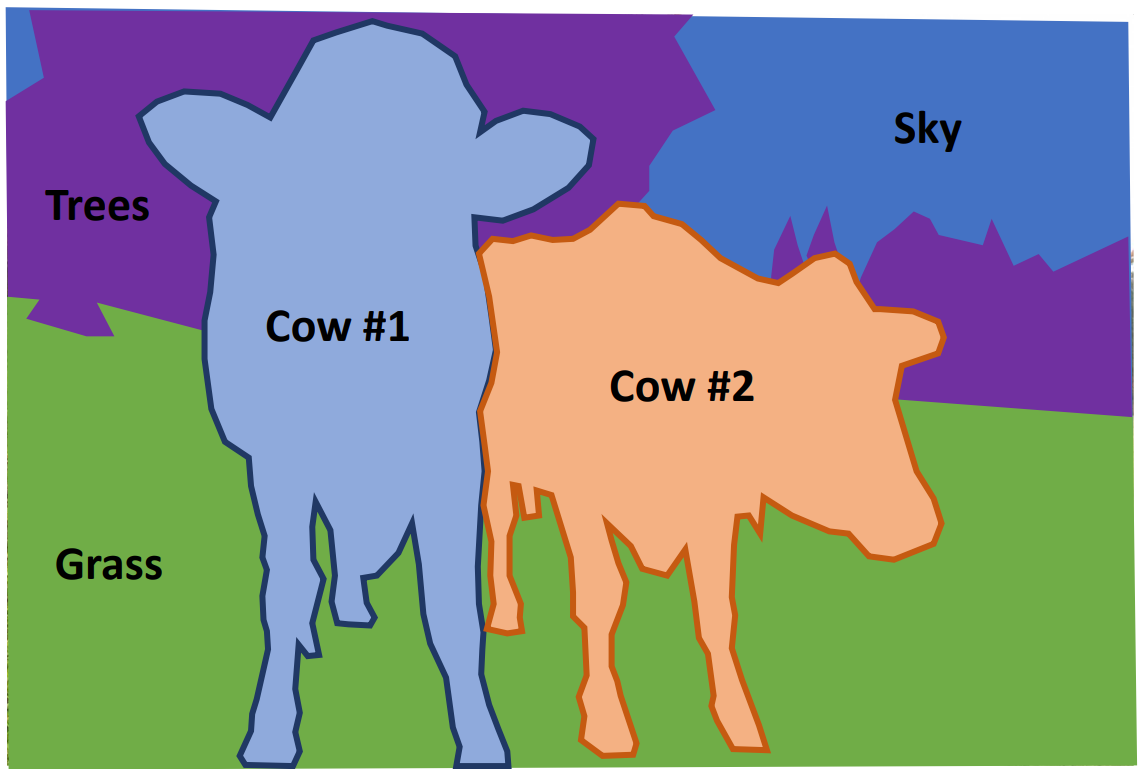
\includegraphics[width=1.0\textwidth,height=1.0\textheight,keepaspectratio]{images/segmentation/ins_10.png}
        \end{figure}
    \end{column}
    \end{columns}
}

\only<2>{
\begin{figure}
\centering
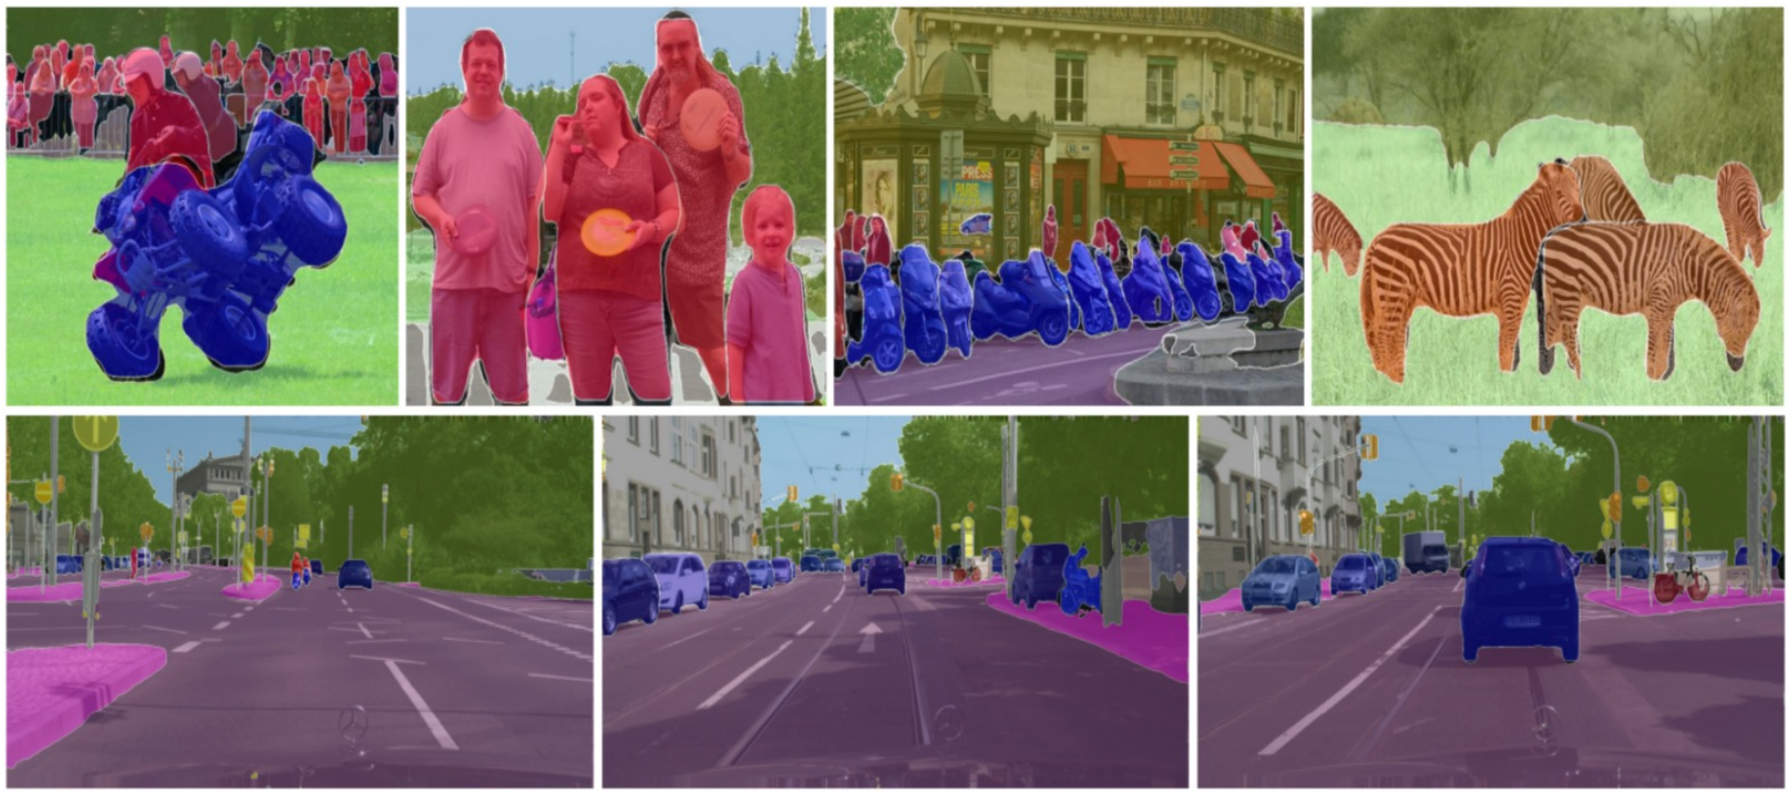
\includegraphics[width=1.0\textwidth,height=1.0\textheight,keepaspectratio]{images/segmentation/ins_11.png}
\footnotetext{Kirillov et al, “Panoptic Feature Pyramid Networks”, CVPR 2019}
\end{figure}
}
\end{frame}